% !TEX program = pdflatex
% !TEX options = -synctex=1 -interaction=nonstopmode -file-line-error "%DOC%"
% 固体物理第一次作业
\documentclass[UTF8,10pt,a4paper]{article}
\usepackage{ctex}
% \catcode`\。=\active
% \newcommand{。}{.}
\newcommand{\CourseName}{固体物理}
\newcommand{\CourseCode}{PHYS1502}
\newcommand{\Semester}{2019-2020学年第二学期}
\newcommand{\ProjectName}{第一次作业}
\newcommand{\DueTimeType}{截止时间}
\newcommand{\DueTime}{2020. 3. 13(周五)17:00}
\newcommand{\StudentName}{陈稼霖}
\newcommand{\StudentID}{45875852}
\usepackage[vmargin=1in,hmargin=.5in]{geometry}
\usepackage{fancyhdr}
\usepackage{lastpage}
\usepackage{calc}
\pagestyle{fancy}
\fancyhf{}
\fancyhead[L]{\CourseName}
\fancyhead[C]{\ProjectName}
\fancyhead[R]{\StudentName}
\fancyfoot[R]{\thepage\ / \pageref{LastPage}}
\setlength\headheight{12pt}
\fancypagestyle{FirstPageStyle}{
    \fancyhf{}
    \fancyhead[L]{\CourseName\\
        \CourseCode\\
        \Semester}
    \fancyhead[C]{{\Huge\bfseries\ProjectName}\\
        \DueTimeType\ : \DueTime}
    \fancyhead[R]{姓名 : \makebox[\widthof{\StudentID}][s]{\StudentName}\\
        学号 : \StudentID\\
        成绩 : \underline{\makebox[\widthof{\StudentID}]{}}}
    \fancyfoot[R]{\thepage\ / \pageref{LastPage}}
    \setlength\headheight{36pt}
}
\usepackage{amsmath,amssymb,amsthm,bm}
\allowdisplaybreaks[4]
\newtheoremstyle{Problem}
{}
{}
{}
{}
{\bfseries}
{.}
{ }
{第\thmnumber{ #2}\thmname{ #1}\thmnote{ (#3)} 得分: \underline{\qquad\qquad}}
\theoremstyle{Problem}
\newtheorem{prob}{题}
\newtheoremstyle{Solution}
{}
{}
{}
{}
{\bfseries}
{:}
{ }
{\thmname{#1}}
\makeatletter
\def\@endtheorem{\qed\endtrivlist\@endpefalse}
\makeatother
\theoremstyle{Solution}
\newtheorem*{sol}{解}
\usepackage{graphicx}
\usepackage{booktabs}
\usepackage{listings}
\lstset{
 columns=fixed,
 numbers=left,
 frame=none,
 showstringspaces=false,
 language=fortran,
}
\begin{document}
\thispagestyle{FirstPageStyle}
\begin{prob}[2.1 Einstein Solid]
    \begin{enumerate}
        \item[(a)] \textit{Classical Einstein (or "Boltzmann") Solid:}\\
              Consider a three-dimensional simple harmonic oscillator with mass $m$ and spring constant $k$ (i.e., the mass that attracted to the origin with the same spring constant in all three directions). The Hamiltonian is given in the usual way by
              \[
                  H=\frac{\bm{p}^2}{2m}+\frac{k}{2}\bm{x}^2
              \]
              \begin{itemize}
                  \item[$\triangleright$] Calculate the classical partition function
                        \[
                            Z=\int\frac{\bm{dp}}{(2\pi\hbar)^3}\int\bm{dx}\,e^{-\beta H(\bm{p},\bm{x})}
                        \]
                        Note: in this exercise $\bm{p}$ and $\bm{x}$ are three-dimensional vectors.
                  \item[$\triangleright$] Using the partition function, calculate the heat capacity $3k_B$.
                  \item[$\triangleright$] Conclude that if you can consider a solid to consist of $N$ atoms all in harmonic wells, then the heat capacity should be $3Nk_B=3R$, in agreement with the law of Dulong and Petit.
              \end{itemize}
        \item[(b)] \textit{Quantum Einstein Solid}:\\
              Now consider the same Hamiltonian quantum-mechanically.
              \begin{itemize}
                  \item[$\triangleright$] Calculate the quantum partition function
                        \[
                            Z=\sum_je^{-\beta E_j}
                        \]
                        where the sum over $j$ is a sum over all eigenstates.
                  \item[$\triangleright$] Explain the relationship with Bose statistics.
                  \item[$\triangleright$] Find an expression for the heat capacity.
                  \item[$\triangleright$] Show that the high-temperature limit agrees with the law of Dulong and Petit.
                  \item[$\triangleright$] Sketch the heat capacity as a function of temperature.\\
                        (See also Exercise 2.7 for more on the same topic)
              \end{itemize}
    \end{enumerate}
\end{prob}
\begin{sol}
    \begin{enumerate}
        \item[(a)]
              \begin{itemize}
                  \item[$\triangleright$] 三维简谐振子的经典配分函数为
                        \begin{align}
                            \nonumber Z= & \int\frac{\bm{dp}}{(2\pi\hbar)^3}\int\bm{dx}\,e^{-\beta\left(\frac{\bm{p}^2}{2m}+\frac{k}{2}\bm{x}^2\right)}                                                        \\
                            \nonumber=   & \iiint\frac{dp_x\,dp_y\,dp_z}{(2\pi\hbar)^3}\iiint dx\,dy\,dz\,e^{-\beta\left[\frac{1}{2m}\left(p_x^2+p_y^2+p_z^2\right)+\frac{k}{2}\left(x^2+y^2+z^2\right)\right]} \\
                            =   & \frac{1}{(2\pi\hbar)^3}\left[\sqrt{\frac{2\pi m}{\beta}}\right]^3\left[\sqrt{\frac{2\pi}{\beta k}}\right]^3=\frac{m^{3/2}}{\hbar^3\beta^3k^{3/2}}
                        \end{align}
                  \item[$\triangleright$] 由上面的配分函数,单个谐振子的内能为
                        \begin{equation}
                            U=-\frac{\partial}{\partial\beta}\ln Z=\frac{3}{\beta}=3k_BT.
                        \end{equation}
                        单个谐振子的热容为
                        \begin{equation}
                            C=\frac{\partial U}{\partial T}=3k_B.
                        \end{equation}
                  \item[$\triangleright$] 因热容是广延量,故若将固体中的$N$个原子均视为如上的谐振子,则该固体的热容为$3Nk_B=3R$,符合杜隆-珀蒂定律.
              \end{itemize}
        \item[(b)] \begin{itemize}
                  \item[$\triangleright$] 三维谐振子的各本征态的哈密顿为
                        \begin{equation}
                            H_{n_x,n_y,n_z}=\hbar\omega\left[\left(n_x+\frac{1}{2}\right)+\left(n_y+\frac{1}{2}\right)+\left(n_z+\frac{1}{2}\right)\right]=\hbar\omega,\quad n_x,n_y,n_z=1,2,3,\cdots,
                        \end{equation}
                        其中$\omega=\sqrt{\frac{k}{m}}$.
                        谐振子的量子配分函数为
                        \begin{align}
                            \nonumber Z= & \sum_{n_x,n_y,n_z=1}^{\infty}e^{-\beta H_{n_x,n_y,n_z}}                                                                                                                                                              \\
                            \nonumber=   & \sum_{n_x=1}^{\infty}e^{-\beta\hbar\omega\left(n_x+\frac{1}{2}\right)}\sum_{n_y=1}^{\infty}e^{-\beta\hbar\omega\left(n_y+\frac{1}{2}\right)}\sum_{n_z=1}^{\infty}e^{-\beta\hbar\omega\left(n_z+\frac{1}{2}\right)} \\
                            \nonumber=   & \left(\frac{e^{-\beta\hbar\omega/2}}{1-e^{-\beta\hbar\omega}}\right)^3=\left(\frac{1}{e^{\beta\hbar\omega/2}-e^{-\beta\hbar\omega/2}}\right)^3
                        \end{align}
                  \item[$\triangleright$] 由上面的配分函数,单个谐振子的平均能量为
                        \begin{align}
                            \nonumber\langle E\rangle= & -\frac{\partial}{\partial\beta}\ln Z=\frac{\frac{3}{2}\hbar\omega\left(e^{\beta\hbar\omega/2}+e^{-\beta\hbar\omega/2}\right)}{e^{\beta\hbar\omega/2}-e^{-\beta\hbar\omega/2}}             \\
                            \nonumber=                 & \frac{3}{2}\hbar\omega\frac{e^{\beta\hbar\omega/2}-e^{-\beta\hbar\omega/2}+2e^{-\beta\hbar\omega/2}}{e^{\beta\hbar\omega/2}-e^{-\beta\hbar\omega/2}} \\
                            =                 & 3\hbar\omega\left[\frac{e^{-\beta\hbar\omega/2}}{e^{\beta\hbar\omega/2}-e^{-\beta\hbar\omega/2}}+\frac{1}{2}\right]=3\hbar\omega\left[\frac{1}{e^{\beta\hbar\omega}-1}+\frac{1}{2}\right].
                        \end{align}
                        上式中括号内第一项正好为玻色分布下(一维)谐振子所处的平均能级序号
                        \begin{equation}
                            \langle n\rangle=\frac{1}{e^{\beta\hbar\omega}-1}.
                        \end{equation}
                        也就是说,谐振子的状态分布服从玻色统计,其每个维度上的振动的能级序号平均值为$\langle n\rangle=\frac{1}{e^{\beta\hbar\omega}-1}$,每个维度上的能量为$\hbar\omega\left(\langle n\rangle+\frac{1}{2}\right)$. 由于谐振子在三个维度上做简谐振动,故其能量平均值为
                        \begin{equation}
                            \langle E\rangle=3\hbar\omega\left(\langle n\rangle+\frac{1}{2}\right)
                        \end{equation}
                  \item[$\triangleright$] 单个谐振子的热容为
                        \begin{equation}
                            C=\frac{\partial\langle E\rangle}{\partial T}=3(\hbar\omega)^2\frac{e^{\beta\hbar\omega}}{\left(e^{\beta\hbar\omega}-1\right)^2}\frac{1}{k_BT^2}=3k_B(\beta\hbar\omega)^2\frac{e^{\beta\hbar\omega}}{\left(e^{\beta\hbar\omega}-1\right)^2}.
                        \end{equation}
                  \item[$\triangleright$] 在高温极限下,$\beta\rightarrow 0$,从而热容$C\rightarrow 3k_B$,符合杜隆-珀蒂定律.
                  \item[$\triangleright$] 热容关于温度的函数图像如图\ref{1-C-T}.
                        \begin{figure}[h]
                            \centering
                            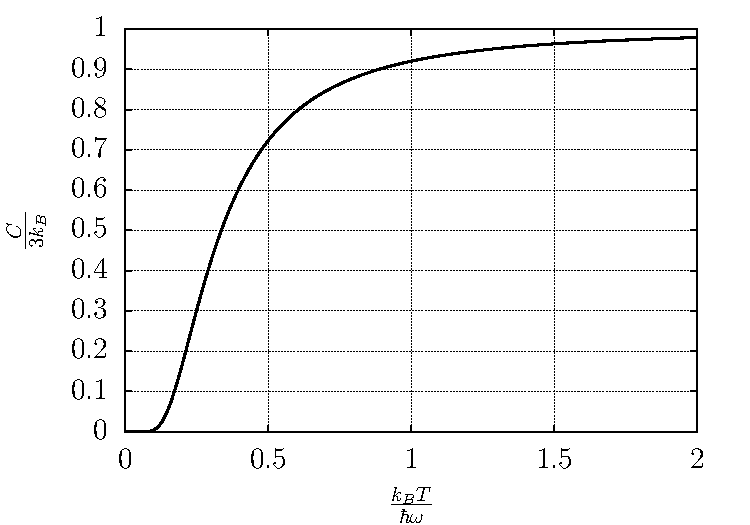
\includegraphics[width=.5\textwidth]{1-C-T.pdf}
                            \caption{热容关于温度的函数图像,其中横坐标温度$T$以$\hbar\omega/k_B$为单位,纵坐标热容$C$以$3k_B$为单位.}
                            \label{1-C-T}
                        \end{figure}
              \end{itemize}
    \end{enumerate}
\end{sol}

\begin{prob}[2.2 Debye Theory I]
    \begin{enumerate}
        \item[(a)$\ddagger$] State the assumption of the Debye model of heat capacity of a solid.
              \begin{itemize}
                  \item[$\triangleright$] Derive the Debye heat capacity as a function of temperature (you will have to leave the final result in terms of an integral that cannot be done analytically).
                  \item[$\triangleright$] From the final result, obtain the high-temperature and low-temperature limits of the heat capacity analytically.\\
                        You may find the following integral to be useful
                        \[
                            \int_0^{\infty}dx\,\frac{x^3}{e^x-1}=\sum_{n=1}^{\infty}\int_0^{\infty}x^3e^{-nx}=6\sum_{n=1}^{\infty}\frac{1}{n^4}=\frac{\pi^4}{15}.
                        \]
                        By integrating by parts this can also be written as
                        \[
                            \int_0^{\infty}dx\,\frac{x^4e^x}{(e^x-1)^2}=\frac{4\pi^4}{15}.
                        \]
              \end{itemize}
        \item[(b)] The following table gives the heat capacity $C$ for potassium iodide as a function fo temperature.
              \begin{table}[h]
                  \centering
                  \begin{tabular}{cc}
                      \toprule
                      $T(\text{K})$ & $C(\text{J K}^{-1}\text{mol}^{-1})$ \\ \midrule
                      $0.1$         & $8.5\times 10^{-7}$                 \\
                      $1.0$         & $8.6\times 10^{-4}$                 \\
                      $5$           & $.12$                               \\
                      $8$           & $.59$                               \\
                      $10$          & $1.1$                               \\
                      $15$          & $2.8$                               \\
                      $20$          & $6.3$                               \\ \bottomrule
                  \end{tabular}
              \end{table}
              \begin{itemize}
                  \item[$\triangleright$] Discuss, with reference to the Debye theory, and make an estimate of the Debye temperature.
              \end{itemize}
    \end{enumerate}
\end{prob}
\begin{sol}
    \begin{enumerate}
        \item[(a)] 德拜的假设:类比光波可以量子化为光子,固体中的声波(机械振动波)可以量子化为声子. 对于给定的波矢$\bm{k}$,声子有三个振动模式(一个纵模+两个横模),具有线性的色散关系:
        \begin{equation}
            \omega=v|\bm{k}|.
        \end{equation}
              \begin{itemize}
                  \item[$\triangleright$] 固体的内能为所有振动模式的能量之和
                        \begin{equation}
                            U=3\sum_{\bm{k}}\hbar\omega(\bm{k})\left(n(\omega)+\frac{1}{2}\right).
                        \end{equation}
                        由Born–von Karman边界条件,波矢的可能大小为
                        \begin{equation}
                            k=\frac{2\pi n}{L},
                        \end{equation}
                        即相邻大小的波矢间隔$\Delta k=\frac{2\pi}{L}$.
                        将上面内能的求和式转化为关于波矢积分:
                        \begin{align}
                            \nonumber U= & 3\int\hbar\omega(\bm{k})\left(n(\omega)+\frac{1}{2}\right)\frac{d\bm{k}}{(\Delta k)^3}                                                                                \\
                            \nonumber=   & 3\frac{L^3}{(2\pi)^3}\int\hbar\omega(\bm{k})\left(n(\omega)+\frac{1}{2}\right)\,d\bm{k}                                                                               \\
                            \nonumber=   & 3\frac{L^3}{(2\pi)^3}\int_0^{2\pi} d\varphi\int_0^{\pi}\sin\theta\,d\theta\int_0^{\omega_{\text{cutoff}}}k^2\hbar\omega(\bm{k})\left(n(\omega)+\frac{1}{2}\right)\,dk \\
                            =            & 3\frac{4\pi L^3}{(2\pi)^3}\int_0^{\omega_{\text{cutoff}}}k^2\hbar\omega(\bm{k})\left(n(\omega)+\frac{1}{2}\right)\,dk.
                        \end{align}
                        其中$\omega_d$是声子频率的上限. 将色散关系代入上式,有
                        \begin{align}
                            \nonumber U= & 3\frac{4\pi L^3}{(2\pi)^3}\int_0^{\omega_{\text{cutoff}}}\left(\frac{\omega}{v}\right)^2\hbar\omega\left(n(\omega)+\frac{1}{2}\right)\,d\left(\frac{\omega}{v}\right) \\
                            \nonumber=   & 3\frac{4\pi L^3\hbar}{(2\pi)^3v^3}\int_0^{\omega_{\text{cutoff}}}\omega^3\left(n(\omega)+\frac{1}{2}\right)\,d\omega                                                  \\
                            =            & \int_0^{\omega_\text{cutoff}}g(\omega)\hbar\omega\left(n(\omega)+\frac{1}{2}\right)\,d\omega,
                        \end{align}
                        其中声子的态密度函数为
                        \begin{equation}
                            g(\omega)=L^3\left[\frac{12\pi\omega^2}{(2\pi)^3v^3}\right]=N\left[\frac{12\pi\omega^2}{(2\pi)^3nv^3}\right]=N\frac{9\omega^2}{\omega_d^3},
                        \end{equation}
                        其中$N$为固体中的原子数,$n=\frac{N}{L^3}$为固体中的原子数密度,德拜温度$\omega_d$满足$\omega_d^3=6\pi^2nv^3$. 由于固体由$N$个自由度为$3$的原子组成,故共有$3N$个振动模式,声子的态密度函数满足
                        \begin{equation}
                            \int_0^{\omega_{\text{cutoff}}}g(\omega)\,d\omega=\frac{3N\omega_{\text{cutoff}}^3}{\omega_d^3}=3N.
                        \end{equation}
                        故
                        \begin{equation}
                            \Longrightarrow\omega_{\text{cutoff}}=\omega_d
                        \end{equation}
                        声子的状态服从玻色分布:
                        \begin{equation}
                            n(\omega)=\frac{1}{e^{\beta\hbar\omega}-1}.
                        \end{equation}
                        故固体的内能为
                        \begin{equation}
                            U=\frac{9N\hbar}{\omega_d^3}\int_0^{\omega_d}\frac{\omega^3}{e^{\beta\hbar\omega}-1}\,d\omega+U_0,
                        \end{equation}
                        其中$U_0$为温度$T=0$时固体的内能,它与$T$无关.
                        令$x=\beta\hbar\omega$,上式可化为
                        \begin{equation}
                            U=\frac{9N\hbar}{\omega_d^3(\beta\hbar)^4}\int_0^{\beta\hbar\omega_d}\frac{x^3}{e^x-1}\,dx+U_0.
                        \end{equation}
                        固体的热容为
                        \begin{equation}
                            \label{2-C}
                            C=\frac{\partial U}{\partial T}=\frac{\partial}{\partial T}\left[\frac{9N\hbar}{\omega_d^3(\beta\hbar)^4}\int_0^{\beta\hbar\omega_d}\frac{x^3}{e^x-1}\,dx\right].
                        \end{equation}
                  \item[$\triangleright$] 在高温极限下,$\beta\rightarrow 0$,故$\frac{1}{e^x-1}=\frac{1}{x}$,从而有
                        \begin{align}
                            \nonumber C= & \frac{\partial}{\partial T}\left[\frac{9N\hbar}{\omega_d^3(\beta\hbar)^4}\int_0^{\beta\hbar\omega_d}x^2\,dx\right]=\frac{\partial}{\partial T}\left[\frac{9N\hbar}{\omega_d^3(\beta\hbar)^4}\frac{1}{3}(\beta\hbar\omega_d)^3\right]=\frac{\partial}{\partial T}\left[3Nk_BT\right]=3Nk_B.
                        \end{align}
                        在低温极限下,$\beta\rightarrow+\infty$,故可将式\eqref{2-C}中的积分上限近似为$+\infty$,从而有
                        \begin{equation}
                            C=\frac{\partial}{\partial T}\left[\frac{9N\hbar}{\omega_d^3(\beta\hbar)^4}\frac{\pi^4}{15}\right]=\frac{\partial}{\partial T}\left[\frac{3\pi^4Nk_B^4T^4}{5\omega_d^3\hbar^3}\right]=\frac{12\pi^4Nk_B^4T^3}{5\omega_d^3\hbar^3}=\frac{12\pi^4Nk_B}{5}\left(\frac{T}{T_{\text{Debye}}}\right)^3,
                        \end{equation}
                        其中德拜温度$T_{\text{Debye}}=\frac{\hbar\omega_d}{k_B}$.
              \end{itemize}
        \item[(b)] 德拜理论表明,在温度接近绝对零度时,固体的热容随温度上升呈三次方形式增长,这与表格中的数据符合得非常好。用最小二乘法拟合表格中的数据(Fortran代码如下)得碘化钾的德拜温度$T_{\text{Debye}}=134$K.
              \begin{lstlisting}
program main
    implicit none
    integer, parameter :: dp = selected_real_kind(8)
    real(dp), parameter :: pi = 3.1415926d0, NA = 6.02214076d23, kB = 1.380649d-23
    integer(1) :: i
    real(dp) :: T(7) = (/.1d0, 1.d0, 5.d0, 8.d0, 10.d0, 15.d0, 20.d0/)
    real(dp) :: C(7) = (/8.5d-7, 8.6d-4, 1.2d-1, 5.9d-1, 1.1d0, 2.8d0, 6.3d0/)
    real(dp) :: TTSum = 0.d0, TCSum = 0.d0, result

    T = T**3
    do i = 1,7
        TTSum = TTSum + T(i)**2
        TCSum = TCSum + T(i) * C(i)
    end do
    result = (12 * pi**4 * NA * kB / (5 * (TCSum / TTSum)))**(1.d0/3.d0)
    write(*,*) result
end program main
            \end{lstlisting}
    \end{enumerate}
\end{sol}

\begin{prob}[Diatomic Einstein Solid*]
    Having studied Exercise 2.1, consider now a solid made up of diatomic molecules. We can (very crudely) model this as two particles in three dimensions, connected to each other with a spring, both in the bottom of a harmonic well.
    \[
        H=\frac{\bm{p_1}^2}{2m_1}+\frac{\bm{p_2}^2}{2m_2}+\frac{k}{2}\bm{x_1}^2+\frac{k}{2}\bm{x_2}^2+\frac{K}{2}(\bm{x_1}-\bm{x_2})^2
    \]
    where $k$ is the spring constant holding both particles in the bottom of the well, and $K$ is the spring constant holding the two particles together. Assume that the two particles are distinguishable atoms.
    (If you find this exercise difficult, for simplicity you may assume that $m_1=m_2$.)
    \begin{enumerate}
        \item[(a)] Analogous to Exercise 2.1, calculate the classical partition function and show that the heat capacity is again $3k_B$ per particle (i.e., $6k_B$ total).
        \item[(b)] Analogous to Exercise 2.1, calculate the quantum partition function and find an expression for the heat capacity. Sketch the heat capacity as a function of temperature if $K\gg k$.
        \item[(c)$^{**}$] How does the result change if the atoms are indistinguishable?
    \end{enumerate}
\end{prob}
\begin{sol}
    \begin{itemize}
        \item[(a)] 双原子分子的经典配分函数为
              \begin{align}
                  \label{3-partition-func}
                  \nonumber Z= & \int\frac{d\bm{p}_1}{(2\pi\hbar)^2}\int\frac{d\bm{p}_2}{(2\pi\hbar)^3}\int d\bm{x}_1\int d\bm{x}_2\,e^{-\beta\left[\frac{\bm{p}_1^2}{2m_1}+\frac{\bm{p}_2^2}{2m_2}+\frac{k}{2}\bm{x}_1^2+\frac{k}{2}\bm{x}_2^2+\frac{K}{2}(\bm{x}_1-\bm{x}_2)^2\right]}                                                \\
                  =            & \frac{1}{(2\pi\hbar)^6}\int d\bm{p}_1\,e^{-\frac{\beta}{2m_1}\bm{p}_1^2}\int d\bm{p}_2\,e^{-\frac{\beta}{2m_2}\bm{p}_2^2}\int d\bm{x}_1\int d\bm{x_2}\,e^{-\beta\left[\frac{k}{2}\bm{x}_1^2+\frac{k}{2}\bm{x}_2^2+\frac{K}{2}(\bm{x}_1-\bm{x}_2)^2\right]},
              \end{align}
              其中
              \begin{align}
                  \label{3-int-p1}
                  \nonumber\int d\bm{p}_1e^{-\frac{\beta}{2m_1}\bm{p}_1^2}= & \int_{-\infty}^{+\infty}dp_{1x}\int_{-\infty}^{+\infty}dp_{1y}\int_{-\infty}^{+\infty}dp_{1z}\,e^{-\frac{\beta}{2m_1}(p_{1x}^2+p_{1y}^2+p_{1z}^2)}                                               \\
                  \nonumber=                                                & \int_{-\infty}^{+\infty}dp_{1x}\,e^{-\frac{\beta}{2m_1}p_{1x}^2}\int_{-\infty}^{+\infty}dp_{1y}\,e^{-\frac{\beta}{2m_1}p_{1y}^2}\int_{-\infty}^{+\infty}dp_{1z}\,e^{-\frac{\beta}{2m_1}p_{1z}^2} \\
                  =                                                         & \left(\frac{2\pi m_1}{\beta}\right)^{3/2},
              \end{align}
              同理
              \begin{equation}
                  \label{3-int-p2}
                  \int d\bm{p}_2\,e^{-\frac{\beta}{2m_2}\bm{p}_2^2}=\left(\frac{2\pi m_2}{\beta}\right)^{3/2}.
              \end{equation}
              做变量代换$\left\{\begin{array}{l}\bm{x}_c=\frac{1}{2}(\bm{x}_1+\bm{x}_2)\\\bm{x}_r=(\bm{x}_1-\bm{x}_2)\end{array}\right.$,即$\left\{\begin{array}{l}\bm{x}_1=\bm{x}_c+\frac{1}{2}\bm{x}_r\\\bm{x}_2=\bm{x}_c-\frac{1}{2}\bm{x}_r\end{array}\right.$,则
              \begin{align}
                  \label{3-int-x1x2}
                  \nonumber  & \int d\bm{x}_1\int d\bm{x}_2\,e^{-\beta\left[\frac{k}{2}\bm{x}_1^2+\frac{k}{2}\bm{x}_2^2+\frac{K}{2}(\bm{x}_1-\bm{x}_2)^2\right]}                                                                                                                                                                                \\
                  \nonumber= & \int d\bm{x}_c\int d\bm{x}_r\,e^{-\beta\left[k\bm{x}_c^2+\left(\frac{k}{4}+\frac{K}{2}\right)\bm{x}_r^2\right]}                                                                                                                                                                                                  \\
                  \nonumber= & \int d\bm{x}_c\,e^{-\beta k\bm{x}_c^2}\int d\bm{x}_r\,e^{-\beta\left(\frac{k}{4}+\frac{K}{2}\right)\bm{x}_r^2}                                                                                                                                                                                                   \\
                  \nonumber= & \int_{-\infty}^{+\infty}dx_{cx}\int_{-\infty}^{+\infty}dx_{cy}\int_{-\infty}^{+\infty}dx_{cz}\,e^{-\beta k(x_{cx}^2+x_{cy}^2+x_{cz}^2)}\int_{-\infty}^{+\infty}dx_{rx}\int_{-\infty}^{+\infty}dx_{ry}\int_{-\infty}^{+\infty}dx_{rz}\,e^{-\beta\left(\frac{k}{4}+\frac{K}{2}\right)(x_{rx}^2+x_{ry}^2+x_{rz}^2)} \\
                  \nonumber= & \int_{-\infty}^{+\infty}dx_{cx}\,e^{-\beta kx_{cx}}\int_{-\infty}^{+\infty}dx_{cy}\,e^{-\beta kx_{cy}^2}\int_{-\infty}^{+\infty}dx_{cz}\,e^{-\beta kx_{cz}^2}                                                                                                                                                    \\
                  \nonumber  & \int_{-\infty}^{+\infty}dx_{rx}\,e^{-\beta\left(\frac{k}{4}+\frac{K}{2}\right)x_{rx}^2}\int_{-\infty}^{+\infty}dx_{ry}\,e^{-\beta\left(\frac{k}{4}+\frac{K}{2}\right)x_{rz}^2}\int_{-\infty}^{+\infty}dx_{rz}\,e^{-\beta\left(\frac{k}{4}+\frac{K}{2}\right)x_{rz}^2}                                            \\
                  =          & \left(\frac{\pi}{\beta k}\right)^{3/2}\left[\frac{\pi}{\beta\left(\frac{k}{4}+\frac{K}{2}\right)}\right]^{3/2}.
              \end{align}
              将式\eqref{3-int-p1}\eqref{3-int-p2}\eqref{3-int-x1x2}代入式\eqref{3-partition-func}中得双原子分子的经典配分函数为
              \begin{equation}
                  Z=\frac{1}{\beta^6}\left[\frac{m_1m_2}{k\left(k+2K\right)}\right]^{3/2}.
              \end{equation}
              单个双原子分子的平均能量为
              \begin{equation}
                  \langle E\rangle=-\frac{\partial}{\partial\beta}\ln Z=\frac{6}{\beta}=6k_BT.
              \end{equation}
              单个双原子分子的热容为
              \begin{equation}
                  C=\frac{\partial\langle E\rangle}{\partial T}=6k_B.
              \end{equation}
              也就是说单个原子的平均热容为$3k_B$.
        \item[(b)] 简单起见,假设$m_1=m_2=m$。做变量代换$\left\{\begin{array}{l}\bm{x}_c=\frac{1}{2}(\bm{x}_1+\bm{x}_2)\\\bm{x}_r=(\bm{x}_1-\bm{x}_2)\\\bm{p}_c=\frac{1}{2}(\bm{p}_1+\bm{p}_2)\\\bm{p}_r=(\bm{p}_1-\bm{p}_2)\end{array}\right.$,即$\left\{\begin{array}{l}\bm{x}_1=\bm{x}_c+\frac{1}{2}\bm{x}_r\\\bm{x}_2=\bm{x}_c-\frac{1}{2}\bm{x}_r\\\bm{p}_1=\bm{p}_c+\frac{1}{2}\bm{p}_r\\\bm{p}_2=\bm{p}_r-\frac{1}{2}\bm{p}_r\end{array}\right.$,则双原子分子的经典哈密顿可化为
              \begin{align}
                  \nonumber H= & \frac{\left(\bm{p}_c+\frac{1}{2}\bm{p}_r\right)^2}{2m}+\frac{\left(\bm{p}_c-\frac{1}{2}\bm{p}_r\right)^2}{2m}+\frac{k}{2}\left(\bm{x}_c+\frac{1}{2}\bm{x}_r\right)^2+\frac{k}{2}\left(\bm{x}_c-\frac{1}{2}\bm{x}_r\right)^2+\frac{K}{2}\bm{x}_r^2 \\
                  =            & \frac{\bm{p}_c^2}{2(m/2)}+\frac{\bm{p}_r^2}{2(2m)}+\frac{(2k)}{2}\bm{x}_c^2+\frac{\left(\frac{k}{2}+K\right)}{2}\bm{x}_r^2.
              \end{align}
              故双原子分子的各本征态的哈密顿可表示为
              \begin{multline}
                  H_{n_{c1},n_{c2},n_{c3},n_{r1},n_{r2},n_{r3}}=\hbar\omega_c\left[\left(n_{c1}+\frac{1}{2}\right)+\left(n_{c2}+\frac{1}{2}\right)+\left(n_{c3}+\frac{1}{2}\right)\right]\\
                  +\hbar\omega_r\left[\left(n_{r1}+\frac{1}{2}\right)+\left(n_{r2}+\frac{1}{2}\right)+\left(n_{r3}+\frac{1}{2}\right)\right],n_{c1},n_{c2},n_{c3},n_{r1},n_{r2},n_{r3}=1,2,3,\cdots.
              \end{multline}
              其中$\omega_c=\sqrt{\frac{4k}{m}}$,$\omega_r=\sqrt{\frac{k+2K}{4m}}$. 双原子分子的量子配分函数为
              \begin{align}
                  \nonumber Z=&\sum_{n_{c1},n_{c2},n_{c3},n_{r1},n_{r2},n_{r3}}^{\infty}e^{-\beta H_{n_{c1},n_{c2},n_{c3},n_{r1},n_{r2},n_{r3}}}\\
                  \nonumber=&\sum_{n_{c1}=1}^{\infty}e^{-\beta\hbar\omega_c\left(n_{c1}+\frac{1}{2}\right)}\sum_{n_{c2}=1}^{\infty}e^{-\beta\hbar\omega_c\left(n_{c2}+\frac{1}{2}\right)}\sum_{n_{c3}=1}^{\infty}e^{-\beta\hbar\omega_c\left(n_{c3}+\frac{1}{2}\right)}\\
                  \nonumber&\sum_{n_{r1}=1}^{\infty}e^{-\beta\hbar\omega_r\left(n_{r1}+\frac{1}{2}\right)}\sum_{n_{r2}=1}^{\infty}e^{-\beta\hbar\omega_r\left(n_{r2}+\frac{1}{2}\right)}\sum_{n_{r3}=1}^{\infty}e^{-\beta\hbar\omega_r\left(n_{r3}+\frac{1}{2}\right)}\\
                  =&\left(\frac{e^{-\beta\hbar\omega_c/2}}{1-e^{-\beta\hbar\omega_c}}\right)^3\left(\frac{e^{-\beta\hbar\omega_r/2}}{1-e^{-\beta\hbar\omega_r}}\right)^3=\left(\frac{1}{e^{\beta\hbar\omega_c/2}-e^{-\beta\hbar\omega_c/2}}\right)^3\left(\frac{1}{e^{\beta\hbar\omega_r/2}-e^{-\beta\hbar\omega_r/2}}\right)^3.
              \end{align}
              由上面的配分函数,单个谐振子的平均能量为
              \begin{align}
                \nonumber\langle E\rangle=&-\frac{\partial}{\partial\beta}\ln Z=\frac{\frac{3}{2}\hbar\omega_c\left(e^{\beta\hbar\omega_c}+e^{-\beta\hbar\omega_c/2}\right)}{e^{\beta\hbar\omega_c/2}-e^{-\beta\hbar\omega_c/2}}+\frac{\frac{3}{2}\hbar\omega_r\left(e^{\beta\hbar\omega_r/2}+e^{-\beta\hbar\omega_r/2}\right)}{e^{\beta\hbar\omega_r/2}-e^{-\beta\hbar\omega_r/2}}\\
                \nonumber=&\frac{3}{2}\hbar\omega_c\frac{e^{\beta\hbar\omega_c/2}-e^{-\beta\hbar\omega_c/2}+2e^{-\beta\hbar\omega_c/2}}{e^{\beta\hbar\omega_c/2}-e^{-\beta\hbar\omega_c/2}}+\frac{3}{2}\hbar\omega_r\frac{e^{\beta\hbar\omega_r/2}-e^{-\beta\hbar\omega_r}}{e^{\beta\hbar\omega/2}-e^{-\beta\hbar\omega/2}}\\
                \nonumber=&3\hbar\omega_c\left[\frac{e^{-\beta\hbar\omega_c/2}}{e^{\beta\hbar\omega_c/2}-e^{-\beta\hbar\omega_c/2}}+\frac{1}{2}\right]+3\hbar\omega_r\left[\frac{e^{-\beta\hbar\omega_r/2}}{e^{\beta\hbar\omega_r/2}-e^{\beta\hbar\omega_r/2}}+\frac{1}{2}\right]\\
                =&3\hbar\omega_c\left[\frac{1}{e^{\beta\hbar\omega_c}-1}+\frac{1}{2}\right]+3\hbar\omega_r\left[\frac{1}{e^{\beta\hbar\omega_r}-1}+\frac{1}{2}\right].
              \end{align}
              单个双原子分子的热容为
              \begin{align}
                  \nonumber C=&\frac{\partial\langle E\rangle}{\partial T}=3(\hbar\omega_c)^2\frac{e^{\beta\hbar\omega_c}}{(e^{\beta\hbar\omega_c}-1)^2}\frac{1}{k_BT^2}+3(\hbar\omega_r)^2\frac{e^{\beta\hbar\omega_r}}{(e^{\beta\hbar\omega_r}-1)^2}\frac{1}{k_BT^2}\\
                  =&3k_B\left[(\beta\hbar\omega_c)^2\frac{e^{\beta\hbar\omega_c}}{(e^{\beta\hbar\omega_c}-1)^2}+(\beta\hbar\omega_r)^2\frac{e^{\beta\hbar\omega_r}}{(e^{\beta\hbar\omega_r}-1)^2}\right].
              \end{align}
              若$K\gg k$,则$\omega_c\gg\omega_r$,故设$\omega_c=1\times 10^{13}$Hz,$\omega_r=1\times 10^{14}$Hz,热容关于温度的函数图像如图\ref{3-C-T}.
              \begin{figure}[h]
                  \centering
                  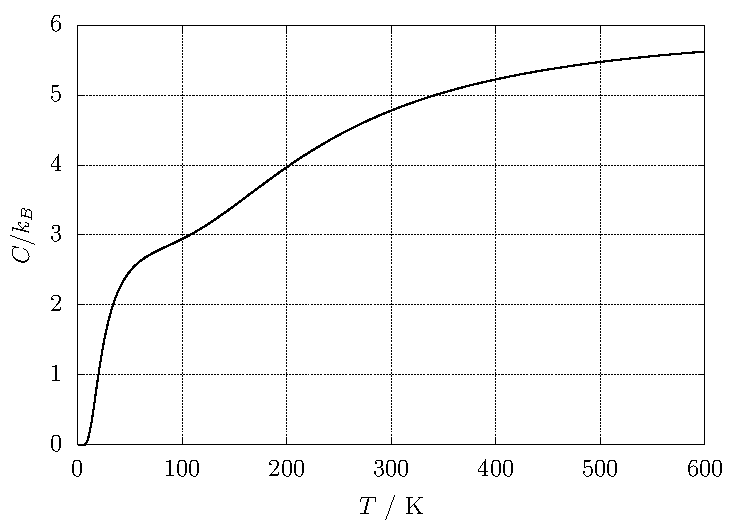
\includegraphics[width=.5\textwidth]{3-C-T.pdf}
                  \caption{热容关于温度的函数图像,其中纵坐标热容$C$以$k_B$为单位.}
                  \label{3-C-T}
              \end{figure}
        \item[(c)] 体系的波函数是两个粒子的波函数的张量积:
        \begin{equation}
            \psi=\psi_1(\bm{x}_1)\otimes\psi_1(\bm{x}_2).
        \end{equation}
        经过$\left\{\begin{array}{l}\bm{x}_c=\frac{1}{2}(\bm{x}_1+\bm{x}_2)\\\bm{x}_r=(\bm{x}_1-\bm{x}_2)\\\bm{p}_c=\frac{1}{2}(\bm{p}_1+\bm{p}_2)\\\bm{p}_r=(\bm{p}_1-\bm{p}_2)\end{array}\right.$的变量代换后,体系的波函数可以化为两个位移矢量分别为$\frac{1}{2}(\bm{x}_1+\bm{x}_2)$和$(\bm{x}_1-\bm{x}_2)$,质量分别为$\frac{m}{2}$和$2m$,劲度系数分别为$2k$和$\frac{k}{2}+K$的谐振子的波函数的张量积:
            \begin{equation}
                \psi=\psi_c(\frac{1}{2}(\bm{x}_1+\bm{x}_2))\otimes\psi(\bm{x}_1-\bm{x}_2).
            \end{equation}
        其中这两个谐振子的波函数又隔可以分解为三个正交方向上的一维谐振子的波函数的张量积:
        \begin{gather}
            \psi_c=\psi_{n_{cx}}\otimes\psi_{n_{cy}}\otimes\psi_{n_{cz}},\\
            \psi_r=\psi_{n_{rx}}\otimes\psi_{n_{ry}}\otimes\psi_{n_{rz}}.
        \end{gather}
        它们对应的能量分别为
        \begin{gather}
            E_c=\hbar\omega_c\left[\left(n_{cx}+\frac{1}{2}\right)+\left(n_{cy}+\frac{1}{2}\right)+\left(n_{cz}+\frac{1}{2}\right)\right],\\
            E_r=\hbar\omega_r\left[\left(n_{rx}+\frac{1}{2}\right)+\left(n_{ry}+\frac{1}{2}\right)+\left(n_{rz}+\frac{1}{2}\right)\right].
        \end{gather}
        $\psi_c(\frac{1}{2}(\bm{x}_1+\bm{x}_2))$不会因两粒子的交换而改变($\psi_c(\bm{x}_1+\bm{x}_2)=\psi_c(\bm{x}_2+\bm{x}_1)$),因此这一部分贡献的热容与此前计算的相同
        \begin{equation}
            C_c=3k_B(\beta\hbar\omega_c)^2\frac{e^{\beta\hbar\omega_c}}{(e^{\beta\hbar\omega_c}-1)^2}.
        \end{equation}
        而$\psi_r(\bm{x}_1+\bm{x}_2)$则需分类讨论.
        假设满足玻色/费米统计,则两个粒子具有交换正/反对称性,即
        \begin{equation}
            \psi_r(\bm{x}_1-\bm{x}_2)=\pm\psi_c(\bm{x}_2-\bm{x}_1).
        \end{equation}
        $\psi_r$为一偶/奇函数,故$\psi_{n_{rx}}$, $\psi_{n_{ry}}$, $\psi_{n_{rx}}$中应当有偶数个奇函数和奇数个偶函数/级数个奇函数和偶数个偶函数,即$n_{rx}+n_{ry}+n_{rz}$为一偶/奇数. $(\bm{x}_1-\bm{x}_2)$对应的谐振子的配分函数为
        \begin{align}
            \nonumber Z_r=&\sum_{(n_{rx}+n_{ry}+n_{rz})\text{ even/odd}}e^{-\beta\hbar\omega_c(n_{rx}+n_{ry}+n_{rz})}\\
            \nonumber=&\frac{1}{2}\sum_{n_{rx},n_{ry},n_{rz}}(1\pm(-1)^{n_{rx}+n_{ry}+n_{rz}})e^{-\beta\hbar\omega_c(n_{rx}+n_{ry}+n_{rz})}\\
            \nonumber=&\frac{1}{2}\left[\left(\frac{1}{e^{\beta\hbar\omega_r/2}-e^{-\beta\hbar\omega_r/2}}\right)^3\right.\\
            \nonumber&\left.+\sum_{n_{rx}=0}^{\infty}(-1)^{n_{rx}}e^{-\beta\hbar\omega_r\left(n_{rx}+\frac{1}{2}\right)}\sum_{n_{ry}=0}^{\infty}(-1)^{n_{ry}}e^{-\beta\hbar\omega_r\left(n_{ry}+\frac{1}{2}\right)}\sum_{n_{rz}=0}^{\infty}(-1)^{n_{rz}}e^{-\beta\hbar\omega_r\left(n_{rz}+\frac{1}{2}\right)}\right]\\
            \nonumber=&\frac{1}{2}\left[\left(\frac{1}{e^{\beta\hbar\omega_r/2}-e^{-\beta\hbar\omega_r/2}}\right)^3\pm\left(\frac{e^{-\beta\hbar\omega_r/2}}{1+e^{-\beta\hbar\omega_r}}\right)^3\right]\\
            =&\frac{1}{2}e^{-3\beta\hbar\omega_r/2}\left[\left(\frac{1}{1-e^{-\beta\hbar\omega_r}}\right)^3\pm\left(\frac{1}{1+e^{-\beta\hbar\omega_r}}\right)^3\right].
        \end{align}
        \textbf{玻色统计下},配分函数可化为
        \begin{equation}
            Z_{r,\text{Bose}}=\frac{e^{-3\beta\hbar\omega_r/2}(1+3e^{-2\beta\hbar\omega_r})}{(1-e^{-\beta\hbar\omega_r})^3(1+e^{-\beta\hbar\omega_r})^3}.
        \end{equation}
        这一振子的平均能量为
        \begin{align}
            \nonumber\langle E\rangle_{r,\text{Bose}}=&-\frac{\partial}{\partial\beta}\ln Z_{r,\text{Bose}}=-\frac{\partial}{\partial\beta}\left[-3\beta\hbar\omega_r/2+\ln(1+3e^{-2\beta\hbar\omega_r})-3\ln(1-e^{-\beta\hbar\omega_r})-3\ln(1+e^{-\hbar\hbar\omega_r})\right]\\
            \nonumber=&3\hbar\omega_r\left(\frac{1}{2}+\frac{2e^{-2\beta\hbar\omega_r}}{1+3e^{-2\beta\hbar\omega_r}}+\frac{e^{-\beta\hbar\omega_r}}{1-e^{-\beta\hbar\omega_r}}-\frac{e^{-\beta\hbar\omega_r}}{1+e^{-\beta\hbar\omega_r}}\right)\\
            =&3\hbar\omega_r\left(\frac{1}{2}+\frac{1}{e^{2\beta\hbar\omega_r}+3}+\frac{1}{e^{\beta\hbar\omega_r}-1}-\frac{1}{e^{\beta\hbar\omega_r}-1}\right).
        \end{align}
        振子的热容为
        \begin{align}
            \nonumber C_{r,\text{Bose}}=&\frac{\partial\langle E\rangle_{r,\text{Bose}}}{\partial T}=3\left(\hbar\omega_r\right)^2\left[\frac{4e^{2\beta\hbar\omega_r}}{(e^{2\beta\hbar\omega_r}+3)^2}+\frac{e^{\beta\hbar\omega_r}}{(e^{\beta\hbar\omega_r}-1)^2}-\frac{e^{\beta\hbar\omega_r}}{(e^{\beta\hbar\omega_r}+1)^2}\right]\frac{1}{k_BT^2}\\
            =&3k_B\left(\beta\hbar\omega_r\right)^2\left[\frac{4e^{2\beta\hbar\omega_r}}{(e^{2\beta\hbar\omega_r}+3)^2}+\frac{e^{\beta\hbar\omega_r}}{(e^{\beta\hbar\omega_r}-1)^2}-\frac{e^{\beta\hbar\omega_r}}{(e^{\beta\hbar\omega_r}+1)^2}\right].
        \end{align}
        故单个分子的热容为
        \begin{equation}
            C_{\text{Bose}}=C_c+C_{r,\text{Bose}}=3k_B\left\{(\beta\hbar\omega_c)^2\frac{e^{\beta\hbar\omega_c}}{(e^{\beta\hbar\omega_c}-1)^2}+\left(\beta\hbar\omega_r\right)^2\left[\frac{4e^{2\beta\hbar\omega_r}}{(e^{2\beta\hbar\omega_r}+3)^2}+\frac{e^{\beta\hbar\omega_r}}{(e^{\beta\hbar\omega_r}-1)^2}-\frac{e^{\beta\hbar\omega_r}}{(e^{\beta\hbar\omega_r}+1)^2}\right]\right\}.
        \end{equation}
        同理,\textbf{费米统计}下,配分函数可化为
        \begin{align}
            \nonumber Z_{r,\text{Fermi}}=&\frac{e^{-3\beta\hbar\omega_r/2}(3e^{-\beta\hbar\omega_r}+e^{-3\beta\hbar\omega_r})}{(1-e^{-\beta\hbar\omega_r})^3(1+e^{-\beta\hbar\omega_r})^3}.
        \end{align}
        这一振子的平均能量为
        \begin{align}
            \nonumber\langle E\rangle_{r,\text{Fermi}}=&-\frac{\partial}{\partial\beta}\ln Z_{r,\text{Fermi}}\\
            \nonumber=&-\frac{\partial}{\partial\beta}\left[-3\beta\hbar\omega_r/2+\ln(3e^{-\beta\hbar\omega_r}+e^{-3\beta\hbar\omega_r})-3\ln(1-e^{-\beta\hbar\omega_r})-3\ln(1+e^{-\beta\hbar\omega_r})\right]\\
            \nonumber=&3\hbar\omega_r\left(\frac{1}{2}+\frac{1+e^{-2\beta\hbar\omega_r}}{3+e^{-2\beta\hbar\omega_r}}+\frac{e^{-\beta\hbar\omega_r}}{1-e^{-\beta\hbar\omega_r}}-\frac{e^{-\beta\hbar\omega_r}}{1+e^{-\beta\hbar\omega_r}}\right)\\
            =&3\hbar\omega_r\left(\frac{1}{2}+\frac{e^{2\beta\hbar\omega_r}+1}{3e^{2\beta\hbar\omega_r}+1}+\frac{1}{e^{\beta\hbar\omega_r}-1}-\frac{1}{e^{\beta\hbar\omega_r}-1}\right).
        \end{align}
        振子的热容为
        \begin{align}
            \nonumber C_{r,\text{Fermi}}=&\frac{\partial\langle E\rangle_{r,\text{Fermi}}}{\partial T}=3(\hbar\omega_r)^2\left[\frac{4e^{2\beta\hbar\omega_r}}{(3e^{2\beta\hbar\omega_r}+1)^2}-\frac{e^{\beta\hbar\omega_r}}{(e^{\beta\hbar\omega_r}-1)^2}-\frac{e^{\beta\hbar\omega}}{e^{\beta\hbar\omega_r}-1}\right]\frac{1}{k_BT^2}\\
            =&3k_B(\beta\hbar\omega_r)^2\left[\frac{4e^{2\beta\hbar\omega_r}}{(3e^{2\beta\hbar\omega_r}+1)^2}-\frac{e^{\beta\hbar\omega_r}}{(e^{\beta\hbar\omega_r}-1)^2}-\frac{e^{\beta\hbar\omega}}{e^{\beta\hbar\omega_r}-1}\right]
        \end{align}
        故单个分子的热容为
        \begin{equation}
            C_{\text{Fermi}}=C_c+C_{r,\text{Fermi}}=3k_B\left\{(\beta\hbar\omega_c)^2\frac{e^{\beta\hbar\omega_c}}{(e^{\beta\hbar\omega_c}-1)^2}+(\beta\hbar\omega_r)^2\left[\frac{4e^{2\beta\hbar\omega_r}}{(3e^{2\beta\hbar\omega_r}+1)^2}-\frac{e^{\beta\hbar\omega_r}}{(e^{\beta\hbar\omega_r}-1)^2}-\frac{e^{\beta\hbar\omega}}{e^{\beta\hbar\omega_r}-1}\right]\right\}.
        \end{equation}
    \end{itemize}
\end{sol}
\end{document}